\chapter{Safety Report}

\section{Introduction}

This document will act as a guide through the entire power distribution and wiring of our rover. All relevant safety measurements to reduce the likelihood of hazards or environmental damages are listed here. 

This document ensures a minimum standard in respect to materialistic and personal safety is defined and taken into account. This not only holds true during the construction but furthermore the actual operation of all the electronics. To illustrate the inner architecture and workings, several schematics, data-sheets and calculations have been created and performed to make this document as comprehensible as possible. 

\section{Hazardous Material List}

Our rover contains 2 lithium-polymer batteries (further named LiPo-batteries) which are
allowable under requirement 1.1 %DATASHEET NEEDED

\section{Power Architecture}



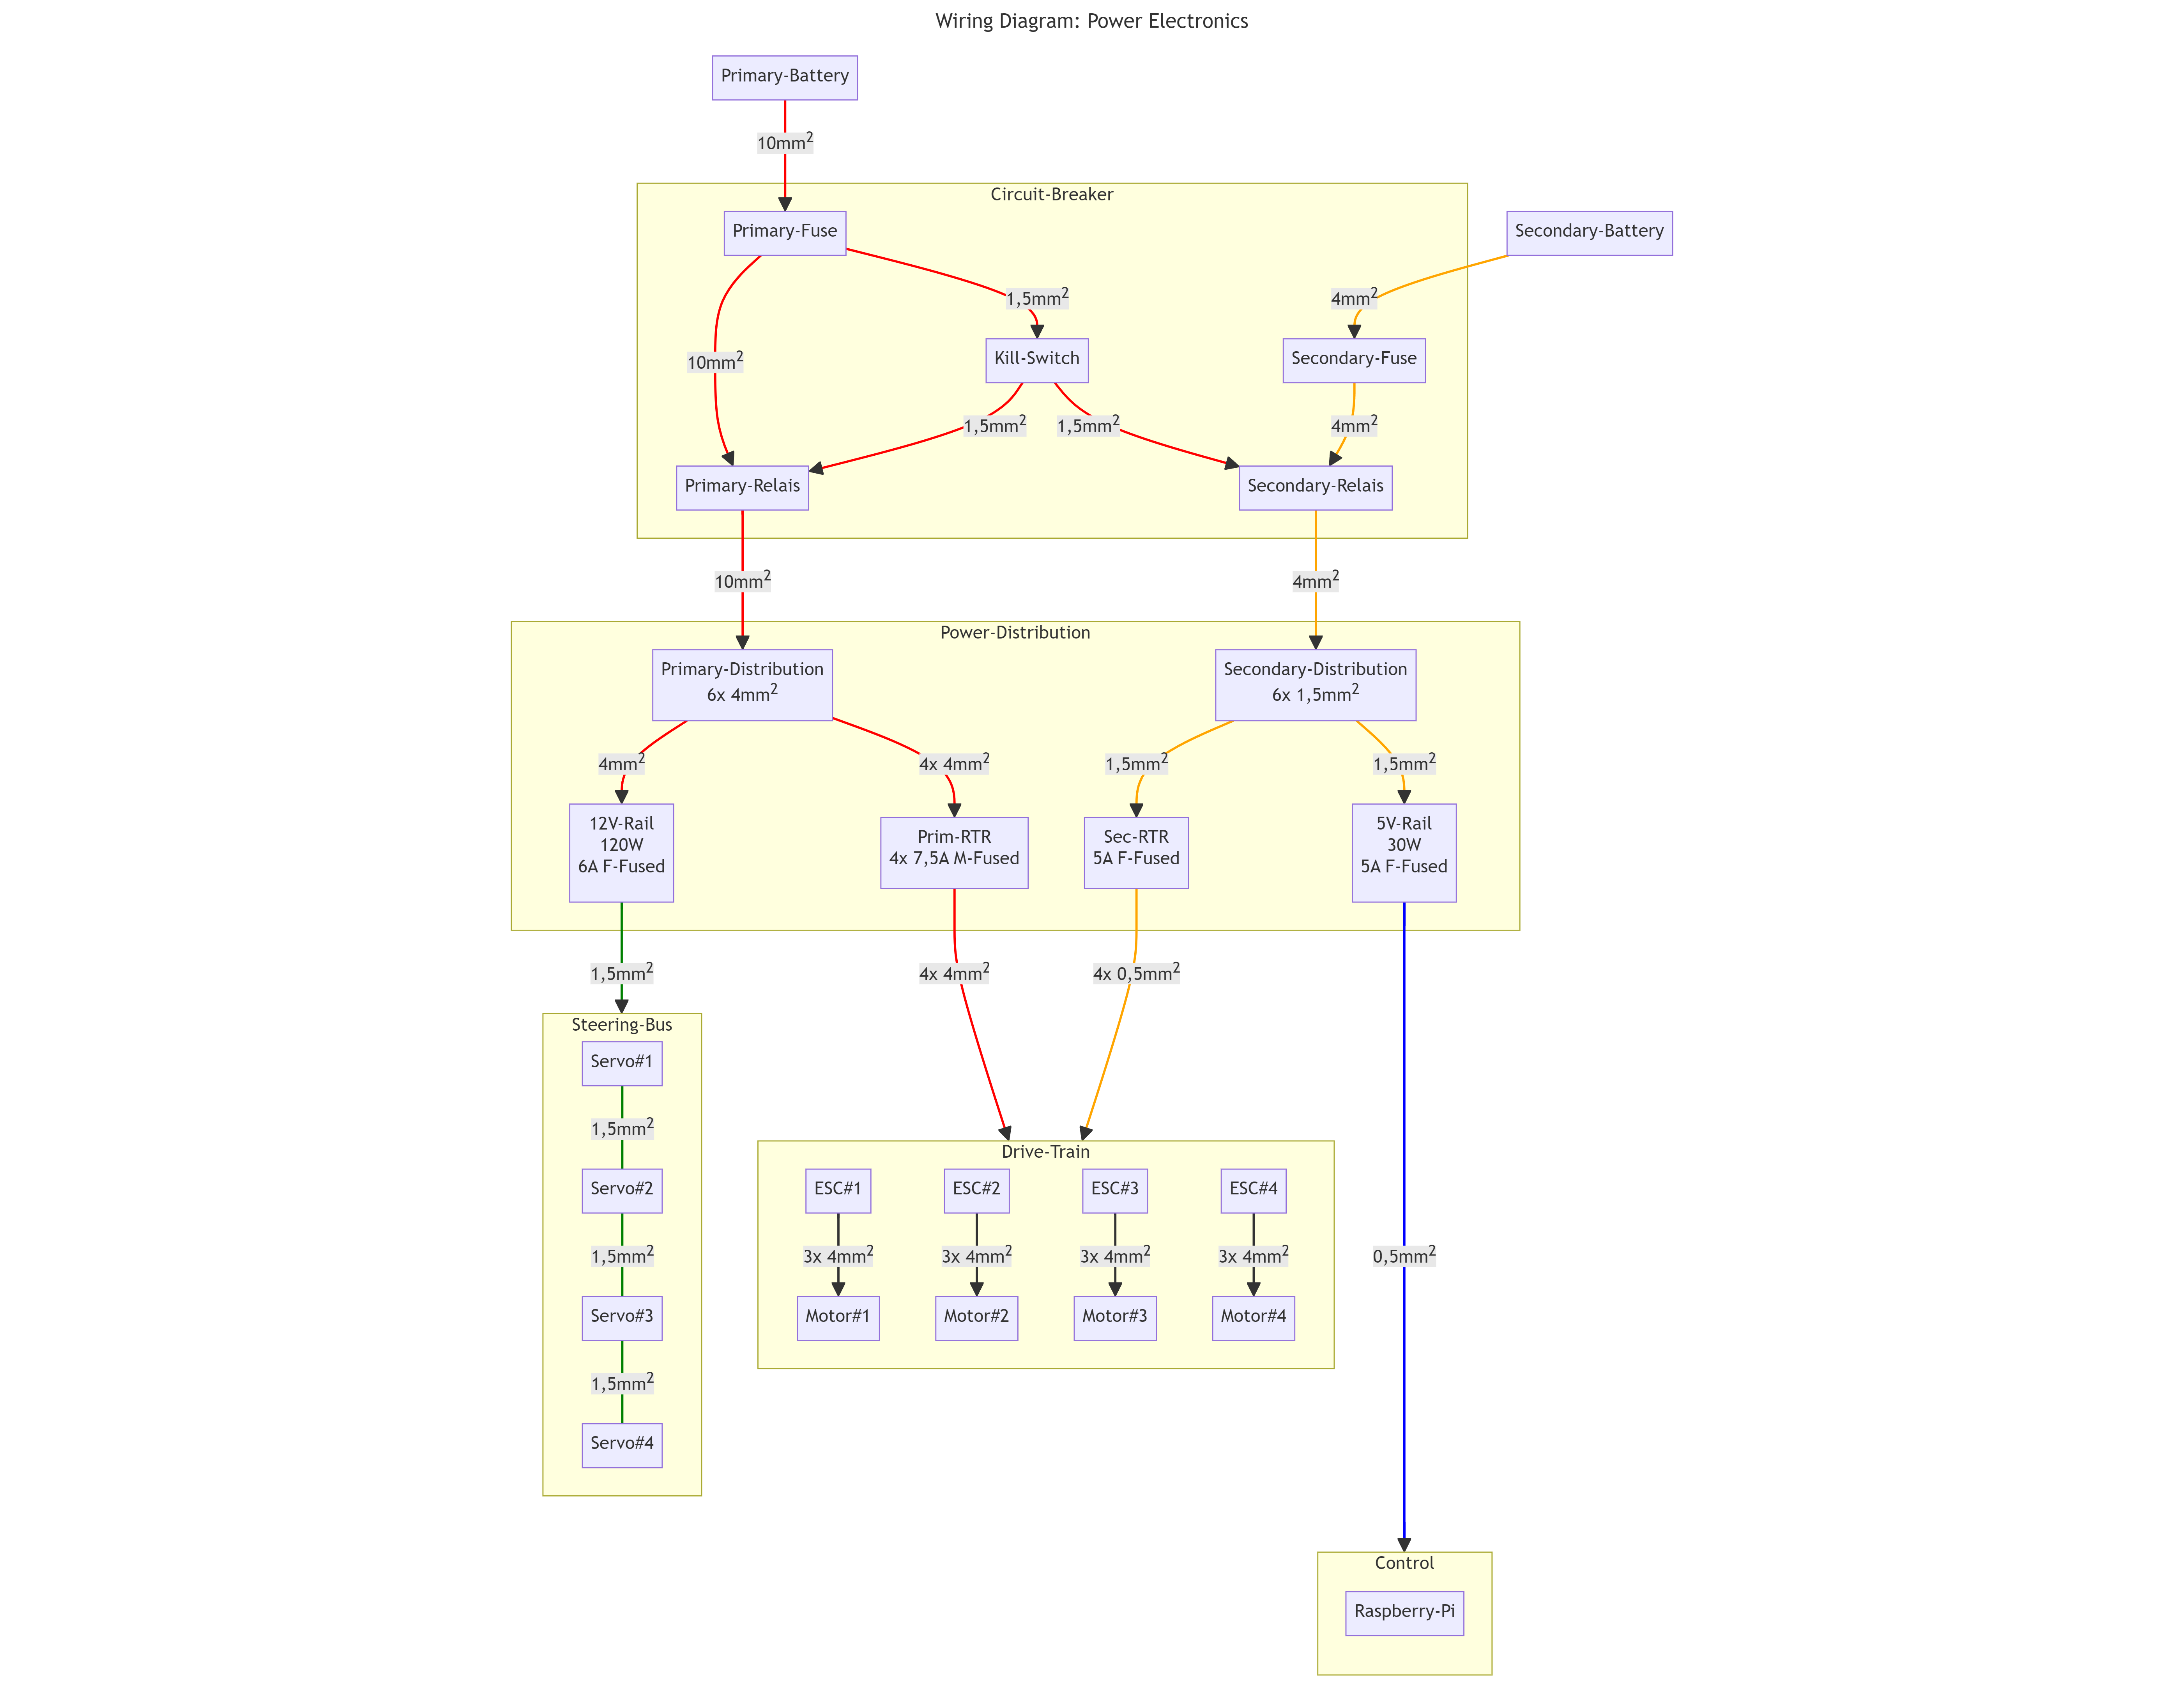
\includegraphics{wiring-power.png}

\section{Energy Storage}

\section{Emergency Stop
}
\section{Power Distribution

\section{Power Conversion}

\section{Power Consuming Circuits}

\section{Unused Circuits}

\section{Circuit Table}




